\documentclass[times, utf8, zavrsni, numeric]{fer}
\usepackage{booktabs}
\usepackage{titlesec}
\newcommand{\sectionbreak}{\clearpage}
\frenchspacing
\begin{document}

% TODO: Navedite broj rada.
\thesisnumber{123456}

\title{Web aplikacija za predstavljanje portfelja programera}

\author{Mislav Vuletić}

\maketitle

\zahvala{}
Posvećeno svima koji su voljni učiti i neprestano napredovati.

\tableofcontents

\chapter{Uvod}
\qquad Prilikom traženja posla prednost je ako se programer može predstaviti potencijalnom poslodavcu sa svim projektima u kojima je sudjelovao i programskom podrškom koju je razvio.
Često se za tu svrhu koriste LinkedIn\footnotemark{} ili Git\footnotemark{} stranice, odnosno druge vlastite web stranice programera.
\footnotetext{LinkedIn - poslovno orijentirana socijalna mreža}
\footnotetext{git - sustav za upravljanje izvornim kodom nastao 2005.~godine}
Učinkovito predstavljanje može se postići uz pomoć jedne web stranice koja će omogućavati pregled projekata kroz Git alate, sadržavati linkove na aktivne projekte te omogućiti međusoban kontakt programera i poslodavca putem korisničkog sučelja.

Ovaj rad prolazi kroz cijeli postupak postavljanja aktivne web stranice programera.

\chapter{Arhitektura}
\section{Korisnici aplikacije}

\chapter{Tehnologije}
\section{Programski jezik Java}
\qquad Java je objektno orijentirani programski jezik razvijen iz programskoj jezika Oak\footnotemark{}.
\footnotetext{Oak - programski jezik razvijen 1991., evoluirao u programski jezik Java 1995.}
Centralna ideja u razvoju programskog jezika Java bila je potpora za više platformnost.
Tako se danas Javin virtualni stroj može vrtiti na gotovo svim platformama; od Linuxa, Solarisa, Mac OS-a do Windowsa.
Druga bitna stavka je da je Java programerima potpuno nebitno hoće li se njihov program izvoditi na 32-bitnom ili 64-bitnom sustavu.
To je zato što Javina specifikacija definira apstraktni računski virtualni stroj kod kojeg je sve propisano.

\section{Java Spring Model-View-Controller}
\qquad Java Spring MVC je modul vrlo popularnog \textit{framework}-a\footnotemark{} Java Spring koji je zaživio u prvom desetljeću 21.~stoljeća.
\footnotetext{framework - radni okvir, definira strukturu, odnosno temelje aplikacije}
Java Spring je \textit{open-source}\footnotemark{} biblioteka za Java platformu.
\footnotetext{open-source - dostupan javnosti na uvid, korištenje, izmjene i daljnju distribuciju}
Omogučava lakši razvoj standardnih i \textit{enterprise}\footnotemark{} aplikacija.
\footnotetext{enterprise aplikacije - prevelika i prekompleksna aplikacija za individualno korištenje}
Java Spring MVC koristi popularnu strategiju izrada web stranica.
MVC definira tri cjeline; \textit{\textbf{M}odel} (model), \textit{\textbf{V}iew} (pogled), \textit{\textbf{C}ontroller} (upravitelj).
\begin{figure}[htb]
				\centering
				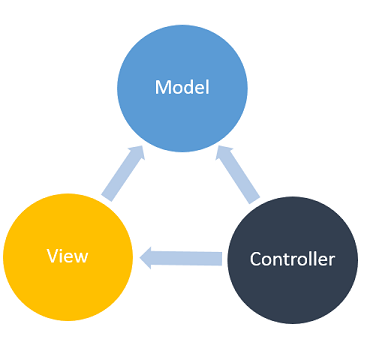
\includegraphics[width=5cm]{images/mvc.png}
				\caption{MVC struktura}
				\label{fig:mvc}
\end{figure}

\noindent
Ideja svake od tih cjelina je jasno odrediti gdje se koji dio aplikacije treba nalaziti.
\begin{itemize}
				\item Model uključuje \textit{backend}\footnotemark{}, te podatke aplikacije, odnosno poslovnu logiku i bazu podataka ako je aplikacija ima.
		\footnotetext{backend - pomoćni sustav, server}
	\item View (pogled) je dio koji korisnik naše aplikacije vidi; 
		html\footnote{html - Hyper Text Markup Language, prezentacijski jezik za izradu web stranica}, 
		css\footnote{css - Cascading Style Sheets, stilski jezik koji služi opisu html dokumenta}, 
		javascript\footnote{javascript - skriptni programski jezik koji se izvršava u web pregledniku}.
	\item Controller (upravitelj) upravlja korisničkim zahtjevima.
\end{itemize}
Dodatno Java Spring definira HandlerAdapter, HandlerInterceptor, HandlerMapping, LocaleResolver, MultipartResolver te ViewResolver koji definiraju gdje se dijelovi koda moraju nalaziti.
\section{Apache}
\qquad Apache server

\section{GitWeb}
\qquad GitWeb

\chapter{Zaključak}
Korištene tehnologije kao Java Spring MVC i ngnix za napravljeni projekt bile su nepotrebne ili bolje reći \textit{overkill}\footnotemark.
\footnotetext{overkill - pretjerano, rušiti dvorac od pijeska buldožerom}

\bibliography{literatura}
\bibliographystyle{fer}
\begin{thebibliography}{9}
\bibitem{}
				Marko Čupić.
				\textit{Programiranje u Javi}.
				Inačica 30. rujna 2015.

\bibitem{awesome-portfolios}
				Awesome Creative Portfolio Websites,
				\\\texttt{github.com/iRaul/awesome-portfolios},
				\\\texttt{www.creative-portfolios.com}

\bibitem{java-spring}
				Spring by Pivotal,
				\\\texttt{spring.io}
\end{thebibliography}

\begin{sazetak}
\qquad Rad predstavlja izradu vlastite web stranice.

\kljucnerijeci{Java, Java Spring, Spring, MVC, portfolio, web, web stranica, portfelj, vlastita web stranica, web stranica programera, javascript}
\end{sazetak}

\engtitle{Software Developer Portfolio Web Application}
\begin{abstract}
Abstract.

\keywords{Java, Java Spring, Spring, MVC, portfolio, web, website, site, developer website, javascript}
\end{abstract}

\end{document}
